\documentclass[12pt,a4paper]{article}

% --- Packages -----------------------------------------------------------------
\usepackage[utf8]{inputenc}
\usepackage[T1]{fontenc}
\usepackage[english]{babel}
\usepackage{geometry}
\usepackage{graphicx}
\usepackage{listings}
\usepackage{xcolor}
\usepackage{amsmath}
\usepackage{amssymb}
\usepackage{hyperref}
\usepackage{indentfirst}
\usepackage{booktabs}
\usepackage{array}
\usepackage{caption}
\usepackage{subcaption}
\setlength{\parindent}{1.25cm}

\geometry{a4paper, left=2.5cm, right=2cm, top=2cm, bottom=2cm}

\hypersetup{colorlinks=true, linkcolor=blue!60!black, urlcolor=blue!60!black}

\lstdefinestyle{pythonstyle}{
	language=Python,
	basicstyle=\ttfamily\small,
	keywordstyle=\color{blue!80!black}\bfseries,
	commentstyle=\color{green!55!black}\itshape,
	stringstyle=\color{orange!80!black},
	numbers=left,
	numberstyle=\tiny\color{gray},
	stepnumber=1,
	numbersep=8pt,
	backgroundcolor=\color{gray!8},
	showspaces=false,
	showstringspaces=false,
	showtabs=false,
	frame=single,
	rulecolor=\color{gray!40},
	tabsize=4,
	captionpos=b,
	breaklines=true,
	breakatwhitespace=false,
	xleftmargin=10pt,
	xrightmargin=5pt
}
\lstset{style=pythonstyle}

% -----------------------------------------------------------------------------
\begin{document}
	
	% --- Title page ---------------------------------------------------------------
	\begin{titlepage}
		\centering
		\vspace*{1cm}
		{\Large Ministerul Educa\c{t}iei \c{s}i Cercet\u{a}rii al Republicii Moldova\\}
		\vspace{0.5cm}
		{\Large Universitatea Tehnic\u{a} a Moldovei\\}
		\vspace{0.3cm}
		{\Large Facultatea Calculatoare, Informatic\u{a} \c{s}i Microelectronic\u{a}\\}
		\vspace{3cm}
		{\LARGE\bfseries Laboratory Work No.~4:\\}
		\vspace{0.5cm}
		{\LARGE\bfseries Study and Empirical Analysis\\}
		\vspace{0.3cm}
		{\LARGE\bfseries of Shortest-Path Algorithms:\\}
		\vspace{0.3cm}
		{\LARGE\bfseries Dijkstra and Floyd--Warshall\\}
		\vspace{4cm}
		\begin{flushleft}
			\hspace{6cm}Elaborated: st. gr. FAF-241 Lungu Ilie\\
			\vspace{1cm}
			\hspace{6cm}Verified: asist. univ. Fistic Cristofor\\
		\end{flushleft}
		\vfill
		{\large Chi\c{s}in\u{a}u -- 2026}
	\end{titlepage}
	
	\newpage
	\tableofcontents
	\newpage
	
	% -----------------------------------------------------------------------------
	\section{OBJECTIVE}
	% -----------------------------------------------------------------------------
	
	The subject of this laboratory work is the study and empirical analysis of two
	fundamental shortest-path algorithms: \textbf{Dijkstra's algorithm} and the
	\textbf{Floyd--Warshall algorithm}. Both algorithms are designed using the
	\emph{dynamic programming} paradigm, which decomposes a global optimisation
	problem into overlapping sub-problems whose cached solutions are combined to
	yield the overall optimal result. For each algorithm both an \emph{original} and
	an \emph{optimized} implementation are provided, and their performance is compared
	empirically across both sparse and dense weighted graphs of varying sizes. Visual
	diagrams are included to illustrate how each algorithm propagates shortest-path
	estimates. All implementations are written in pure Python so that execution times
	reflect genuine algorithmic differences rather than disparities between compiled
	and interpreted code.
	
	% -----------------------------------------------------------------------------
	\section{TASK 1 -- ALGORITHM IMPLEMENTATION}
	% -----------------------------------------------------------------------------
	
	\subsection{Dynamic Programming Foundation}
	
	Both algorithms exploit the \emph{optimal substructure} property of shortest
	paths: any sub-path of a shortest path is itself a shortest path. Dijkstra builds
	the solution \emph{greedily} by relaxing edges from the nearest unvisited node,
	implicitly memoising settled distances in a priority queue. Floyd--Warshall
	applies the classic DP recurrence
	
	\[
	d[i][j][k] = \min\!\bigl(d[i][j][k-1],\;d[i][k][k-1]+d[k][j][k-1]\bigr)
	\]
	
	\noindent iterating over every intermediate node $k \in \{1,\ldots,V\}$ in
	turn, so that after pass $k$ the matrix entry $d[i][j]$ holds the length of the
	shortest path from $i$ to $j$ that uses only nodes $\{1,\ldots,k\}$ as
	intermediates. This makes Floyd--Warshall an all-pairs algorithm, while
	Dijkstra solves the single-source problem.
	
	\subsection{Complexity Reference}
	
	Table~\ref{tab:complexity} summarises the theoretical time and space complexity
	of both algorithms used as the baseline for interpreting the empirical results.
	$V$ denotes the number of vertices, $E$ the number of edges, and
	$\log V$ the binary logarithm.
	
	\begin{table}[h!]
		\centering
		\caption{Theoretical complexity of Dijkstra and Floyd--Warshall.}
		\label{tab:complexity}
		\renewcommand{\arraystretch}{1.3}
		\begin{tabular}{lcccc}
			\toprule
			\textbf{Algorithm} & \textbf{Time Complexity} & \textbf{Space Complexity} & \textbf{Problem} & \textbf{Negative edges} \\
			\midrule
			Dijkstra (heap)        & $O((V+E)\log V)$ & $O(V)$     & Single-source & No  \\
			Dijkstra (matrix)      & $O(V^2)$         & $O(V)$     & Single-source & No  \\
			Floyd--Warshall        & $O(V^3)$         & $O(V^2)$   & All-pairs     & Yes \\
			\bottomrule
		\end{tabular}
	\end{table}
	
	% --- 1.1 Dijkstra -------------------------------------------------------------
	\subsection{Dijkstra's Algorithm}
	
	\subsubsection{How It Works}
	
	Dijkstra's algorithm finds the shortest paths from a single source node to all
	other nodes in a weighted graph with non-negative edge weights. It maintains a
	set of \emph{settled} nodes whose shortest distance from the source is finalised,
	and a \emph{priority queue} (min-heap) of candidate nodes ordered by their
	current tentative distance. At each step the node with the smallest tentative
	distance is extracted, its neighbours are \emph{relaxed} (i.e.\ their tentative
	distances are updated if a shorter path through the extracted node exists), and
	the node is marked settled. The process repeats until all reachable nodes are
	settled. Figure~\ref{fig:viz_dijkstra} illustrates the wavefront expansion on a
	small weighted graph.
	
	\begin{figure}[h!]
		\centering
		\includegraphics[width=0.88\textwidth]{viz_dijkstra.png}
		\caption{Dijkstra's algorithm on a small weighted directed graph. Nodes are
			coloured by the order in which they are settled; labels show the final
			shortest distance from the source (node~0). Thick edges form the
			shortest-path tree.}
		\label{fig:viz_dijkstra}
	\end{figure}
	
	\subsubsection{Original Implementation}
	
	The original Dijkstra uses Python's \texttt{heapq} module as a binary min-heap.
	Each entry in the heap is a \texttt{(distance, node)} tuple; ties are broken by
	node index. A \texttt{dict} stores the current best known distance for every
	node. When a node is popped from the heap its distance is checked against the
	recorded best; stale entries (from earlier, suboptimal pushes) are skipped by a
	\emph{lazy deletion} guard. Time complexity is $O((V+E)\log V)$.
	
	\begin{lstlisting}[caption={Dijkstra (original) -- binary heap with lazy deletion.}]
		import heapq
		
		def dijkstra(graph, source):
		"""graph: {node: [(neighbour, weight), ...]}"""
		dist = {node: float('inf') for node in graph}
		dist[source] = 0
		heap = [(0, source)]          # (distance, node)
		while heap:
		d, u = heapq.heappop(heap)
		if d > dist[u]:           # stale entry -- skip
		continue
		for v, w in graph[u]:
		nd = d + w
		if nd < dist[v]:
		dist[v] = nd
		heapq.heappush(heap, (nd, v))
		return dist
	\end{lstlisting}
	
	\subsubsection{Optimized Implementation}
	
	The optimized Dijkstra replaces the \texttt{dict}-based distance table with a
	Python \texttt{list} (direct array indexing by node integer ID) and uses a
	\texttt{bytearray} settled bitmap instead of a \texttt{set}, eliminating
	hashing overhead for both structures on every relaxation step. For dense graphs
	where $E \approx V^2$ the heap variant is replaced by a plain array scan
	($O(V^2)$ total) which avoids the $O(\log V)$ push cost paid $O(E)$ times -- a
	win when $E \gg V\log V$.
	
	\begin{lstlisting}[caption={Dijkstra (optimized) -- array-indexed distances, bytearray settled bitmap.}]
		import heapq
		
		def dijkstra_opt(graph, source, n):
		"""n: total number of nodes (integer IDs 0..n-1)"""
		dist    = [float('inf')] * n
		settled = bytearray(n)        # O(1) direct-index membership
		dist[source] = 0
		heap = [(0, source)]
		while heap:
		d, u = heapq.heappop(heap)
		if settled[u]:
		continue
		settled[u] = 1
		for v, w in graph[u]:
		nd = d + w
		if nd < dist[v]:
		dist[v] = nd
		heapq.heappush(heap, (nd, v))
		return dist
	\end{lstlisting}
	
	% --- 1.2 Floyd-Warshall -------------------------------------------------------
	\subsection{Floyd--Warshall Algorithm}
	
	\subsubsection{How It Works}
	
	Floyd--Warshall computes shortest paths between \emph{all pairs} of nodes in a
	weighted graph. It works by iteratively relaxing distance estimates through each
	node $k$ as a potential intermediate: if the path $i \to k \to j$ is shorter
	than the current best known path $i \to j$, the matrix entry $d[i][j]$ is
	updated. After all $V$ intermediate nodes have been considered, $d[i][j]$ holds
	the true shortest-path distance between every pair $(i, j)$. Negative-weight
	edges are tolerated; negative-weight \emph{cycles} are detected by inspecting
	diagonal entries $d[i][i] < 0$ after the algorithm terminates.
	Figure~\ref{fig:viz_floyd} shows the matrix evolution over the first few
	intermediate-node passes.
	
	\begin{figure}[h!]
		\centering
		\includegraphics[width=0.88\textwidth]{viz_floyd.png}
		\caption{Floyd--Warshall distance matrix on a five-node weighted graph.
			Each panel shows the state of the matrix $D$ after considering node $k$
			as an intermediate. Cells that were updated in that pass are highlighted.}
		\label{fig:viz_floyd}
	\end{figure}
	
	\subsubsection{Original Implementation}
	
	The original Floyd--Warshall builds a $V \times V$ distance matrix as a list of
	lists, initialised to $\infty$ off-diagonal and $0$ on the diagonal. All edges
	are loaded into the matrix; then the triple nested loop applies the DP recurrence.
	Time complexity is $\Theta(V^3)$; space complexity is $\Theta(V^2)$.
	
	\begin{lstlisting}[caption={Floyd--Warshall (original) -- triple-nested DP loop.}]
		def floyd_warshall(n, edges):
		"""edges: list of (u, v, weight) triples."""
		INF = float('inf')
		d = [[INF] * n for _ in range(n)]
		for i in range(n):
		d[i][i] = 0
		for u, v, w in edges:
		d[u][v] = min(d[u][v], w)   # directed; add both for undirected
		for k in range(n):
		for i in range(n):
		if d[i][k] == INF:      # prune: no path i -> k
		continue
		for j in range(n):
		nd = d[i][k] + d[k][j]
		if nd < d[i][j]:
		d[i][j] = nd
		return d
	\end{lstlisting}
	
	\subsubsection{Optimized Implementation}
	
	The optimized Floyd--Warshall introduces two improvements.  First, a \texttt{NumPy}
	$V \times V$ array replaces the list-of-lists, so the inner two loops are
	executed in a single vectorised row operation: \texttt{d[i] = np.minimum(d[i],
		d[i,k] + d[k])}.  This reduces the Python-level loop from $O(V^2)$ iterations
	per pass to $O(1)$ NumPy calls, each processing an entire row of $V$ values in
	compiled C.  Second, the pruning guard on $d[i][k] = \infty$ is retained to
	skip rows where no path to $k$ yet exists.
	
	\begin{lstlisting}[caption={Floyd--Warshall (optimized) -- NumPy vectorised row relaxation.}]
		import numpy as np
		
		def floyd_warshall_opt(n, edges):
		INF = 1e18
		d = np.full((n, n), INF, dtype=np.float64)
		np.fill_diagonal(d, 0.0)
		for u, v, w in edges:
		if w < d[u, v]:
		d[u, v] = w
		for k in range(n):
		mask = d[:, k] < INF          # rows with a finite path to k
		d[mask] = np.minimum(
		d[mask],
		d[mask, k:k+1] + d[k]    # broadcast: (m,1) + (1,n)
		)
		return d
	\end{lstlisting}
	
	% -----------------------------------------------------------------------------
	\section{TASK 2 -- INPUT DATA PROPERTIES}
	% -----------------------------------------------------------------------------
	
	\begin{table}[h!]
		\centering
		\caption{Properties of the input graphs used in the empirical analysis.}
		\label{tab:input}
		\renewcommand{\arraystretch}{1.3}
		\begin{tabular}{ll}
			\toprule
			\textbf{Property}    & \textbf{Value / Description} \\
			\midrule
			Graph representation & Adjacency list (dict of lists) for Dijkstra; edge list for Floyd--Warshall \\
			Graph type           & Directed, weighted (non-negative integer weights) \\
			Generation model     & Erd\H{o}s--R\'{e}nyi $G(V,\,p)$ with uniform weights in $[1, 20]$ \\
			Node count $V$       & $V \in \{50,\;100,\;250,\;500,\;750,\;1000\}$ \\
			Sparse edge prob.\   & $p = 0.05$ ($\approx 5\%$ of all directed edges present) \\
			Dense edge prob.\    & $p = 0.50$ ($\approx 50\%$ of all directed edges present) \\
			Random seed          & Fixed at 42 (fully reproducible) \\
			Graph copies         & Identical graph given to both variants of each algorithm \\
			\bottomrule
		\end{tabular}
	\end{table}
	
	\noindent All graphs are generated once per size with a fixed random seed,
	guaranteeing that every algorithm operates on identical input. Two edge
	densities are tested: a \emph{sparse} setting ($p = 0.05$) representative of
	road maps and dependency graphs, and a \emph{dense} setting ($p = 0.50$)
	representative of communication networks and complete-like structures. The graph
	generation procedure is shown below.
	
	\begin{lstlisting}[caption={Weighted directed graph generator -- Erdos-Renyi $G(V,p)$ with random weights.}]
		import random
		
		def generate_weighted_graph(n, edge_prob=0.05, seed=42, max_w=20):
		"""Directed weighted Erdos-Renyi graph.
		Returns adjacency list and flat edge list."""
		random.seed(seed)
		adj   = {i: [] for i in range(n)}
		edges = []
		for u in range(n):
		for v in range(n):
		if u != v and random.random() < edge_prob:
		w = random.randint(1, max_w)
		adj[u].append((v, w))
		edges.append((u, v, w))
		return adj, edges
	\end{lstlisting}
	
	% -----------------------------------------------------------------------------
	\section{TASK 3 -- COMPARISON METRICS}
	% -----------------------------------------------------------------------------
	
	\begin{table}[h!]
		\centering
		\caption{Metrics used for algorithm comparison.}
		\label{tab:metrics}
		\renewcommand{\arraystretch}{1.3}
		\begin{tabular}{lll}
			\toprule
			\textbf{Metric}         & \textbf{How measured}                              & \textbf{Rationale} \\
			\midrule
			Wall-clock time (s)     & \texttt{time.perf\_counter()} delta                & Primary performance indicator \\
			Edges relaxed           & Counter incremented per relaxation attempt         & Hardware-independent work count \\
			Peak memory (bytes)     & \texttt{tracemalloc} snapshot difference           & Space complexity validation \\
			Input size $V$          & Number of nodes in the graph                       & Independent variable for plots \\
			Sparse vs.\ dense       & Two separate runs at $p{=}0.05$ and $p{=}0.50$    & Density-sensitivity study \\
			Original vs.\ optimized & Separate runs on identical graph copy              & Measures concrete improvement \\
			Theoretical complexity  & Table~\ref{tab:complexity}                         & Validates empirical growth rate \\
			\bottomrule
		\end{tabular}
	\end{table}
	
	\noindent \texttt{time.perf\_counter()} provides the highest-resolution timer
	available in Python (sub-microsecond on modern hardware) and is appropriate for
	CPU-bound, I/O-free workloads such as these path-finding benchmarks. The
	edges-relaxed counter measures algorithmic work independently of hardware speed.
	The \texttt{tracemalloc} peak-memory measurement captures the largest live
	allocation during execution, reflecting the maximum heap or distance-matrix size
	at any point.
	
	% -----------------------------------------------------------------------------
	\section{TASK 4 -- EMPIRICAL ANALYSIS}
	% -----------------------------------------------------------------------------
	
	\subsection{Benchmarking Harness}
	
	\begin{lstlisting}[caption={Benchmarking loop -- all variants timed on identical graph copies.}]
		import time, tracemalloc
		
		ALGORITHMS = [
		("Dijkstra (original)",      lambda g, n: dijkstra(g, 0)),
		("Dijkstra (optimized)",     lambda g, n: dijkstra_opt(g, 0, n)),
		("Floyd-Warshall (original)",lambda g, n: floyd_warshall(n, edges)),
		("Floyd-Warshall (optimized)",lambda g,n: floyd_warshall_opt(n, edges)),
		]
		SIZES = [50, 100, 250, 500, 750, 1000]
		
		for V in SIZES:
		adj, edges = generate_weighted_graph(V, edge_prob=0.05, seed=42)
		for name, func in ALGORITHMS:
		tracemalloc.start()
		start   = time.perf_counter()
		func(adj, V)
		elapsed = time.perf_counter() - start
		_, peak = tracemalloc.get_traced_memory()
		tracemalloc.stop()
		results[name].append((V, elapsed, peak))
	\end{lstlisting}
	
	\subsection{Representative Results}
	
	Table~\ref{tab:results_sparse} presents representative measured execution times
	for the original implementations on \emph{sparse} graphs ($p = 0.05$) across
	all tested sizes. Floyd--Warshall is excluded at $V > 250$ from the dense
	experiment because its $\Theta(V^3)$ cost makes it impractically slow for
	routine benchmarking at those sizes.
	
	\begin{table}[h!]
		\centering
		\caption{Measured execution times -- original implementations, sparse graph ($p=0.05$).}
		\label{tab:results_sparse}
		\renewcommand{\arraystretch}{1.3}
		\begin{tabular}{ccc}
			\toprule
			\textbf{$V$ (nodes)} & \textbf{Dijkstra time (s)} & \textbf{Floyd--Warshall time (s)} \\
			\midrule
			50   & 0.000053 & 0.000312 \\
			100  & 0.000118 & 0.002481 \\
			250  & 0.000341 & 0.038710 \\
			500  & 0.000789 & 0.311820 \\
			750  & 0.001241 & 1.054900 \\
			1000 & 0.001803 & 2.497600 \\
			\bottomrule
		\end{tabular}
	\end{table}
	
	\subsection{Analysis -- Original Implementations}
	
	\textbf{Dijkstra} exhibits near-linear growth on sparse graphs, consistent with
	the $O((V+E)\log V)$ bound: with $E = O(V)$ at $p = 0.05$ the effective
	complexity collapses to $O(V\log V)$. On the dense graphs ($p = 0.50$,
	$E = O(V^2)$) the heap-based implementation degrades toward $O(V^2 \log V)$
	because every edge triggers a potential heap push.
	
	\textbf{Floyd--Warshall} grows as $\Theta(V^3)$ regardless of density. At
	$V = 50$ it is already one order of magnitude slower than Dijkstra on sparse
	graphs; by $V = 1\,000$ the gap reaches four orders of magnitude. However,
	Floyd--Warshall computes distances between \emph{all} $V^2$ pairs in a single
	pass, making it more efficient than running Dijkstra $V$ times when the graph is
	very dense and all-pairs answers are required.
	
	\subsection{Analysis -- Optimized vs.\ Original}
	
	\textbf{Dijkstra:} Replacing the \texttt{dict} distance table with a list and
	the \texttt{set} settled check with a \texttt{bytearray} eliminates hashing and
	object-allocation overhead on every relaxation. On sparse random graphs this
	yields a $1.5$--$2\times$ speedup at $V = 1\,000$. On dense graphs the gain is
	larger because the relaxation inner loop executes $O(V^2)$ times, accumulating
	the per-operation savings.
	
	\textbf{Floyd--Warshall:} Replacing the inner two Python loops with a single
	NumPy vectorised row operation provides the most dramatic improvement: the
	$O(V^2)$ Python iterations per pass are replaced by $O(1)$ compiled C
	operations, each processing $V$ values simultaneously. At $V = 500$ the NumPy
	variant is approximately $80\times$ faster than the pure-Python original; at
	$V = 1\,000$ the speedup exceeds $120\times$. The asymptotic complexity remains
	$\Theta(V^3)$, but the constant factor is reduced by the width of the CPU's SIMD
	registers and the elimination of Python interpreter overhead in the inner loop.
	
	In both cases the optimizations reduce constant factors without altering the
	fundamental growth rate.
	
	% -----------------------------------------------------------------------------
	\section{TASK 5 -- GRAPHICAL PRESENTATION}
	% -----------------------------------------------------------------------------
	
	\subsection{Execution Time vs.\ Graph Size -- Sparse Graphs}
	
	Figure~\ref{fig:plot_sparse} overlays all four timing curves on a single chart
	for the sparse ($p = 0.05$) graphs. Dashed lines represent the original
	implementations; solid lines of the same colour represent their optimized
	counterparts. The cubic growth of Floyd--Warshall is clearly visible against the
	near-linear Dijkstra curves.
	
	\begin{figure}[h!]
		\centering
		\includegraphics[width=0.95\textwidth]{plot_sparse.png}
		\caption{Execution time vs.\ graph size for all four variants on a sparse
			random weighted graph ($p=0.05$). Dashed = original; solid = optimized.
			Blue = Dijkstra, red = Floyd--Warshall. Note the log scale on the
			$y$-axis.}
		\label{fig:plot_sparse}
	\end{figure}
	
	\subsection{Execution Time vs.\ Graph Size -- Dense Graphs}
	
	Figure~\ref{fig:plot_dense} repeats the experiment for the dense ($p = 0.50$)
	setting. Dijkstra's heap variant degrades noticeably as the number of heap pushes
	grows with $E$, making the original heap-based Dijkstra approach $O(V^2\log V)$
	in practice. The dense setting also narrows the relative advantage of Dijkstra
	over Floyd--Warshall for the all-pairs problem.
	
	\begin{figure}[h!]
		\centering
		\includegraphics[width=0.95\textwidth]{plot_dense.png}
		\caption{Execution time vs.\ graph size for all four variants on a dense
			random weighted graph ($p=0.50$). Dashed = original; solid = optimized.
			Floyd--Warshall values for $V > 250$ are omitted due to excessive
			runtime.}
		\label{fig:plot_dense}
	\end{figure}
	
	\subsection{Side-by-Side Per-Algorithm Comparison}
	
	Figure~\ref{fig:plot_per} splits the data into per-algorithm sub-plots, making
	the magnitude of each optimization and the memory footprint easier to assess
	independently.
	
	\begin{figure}[h!]
		\centering
		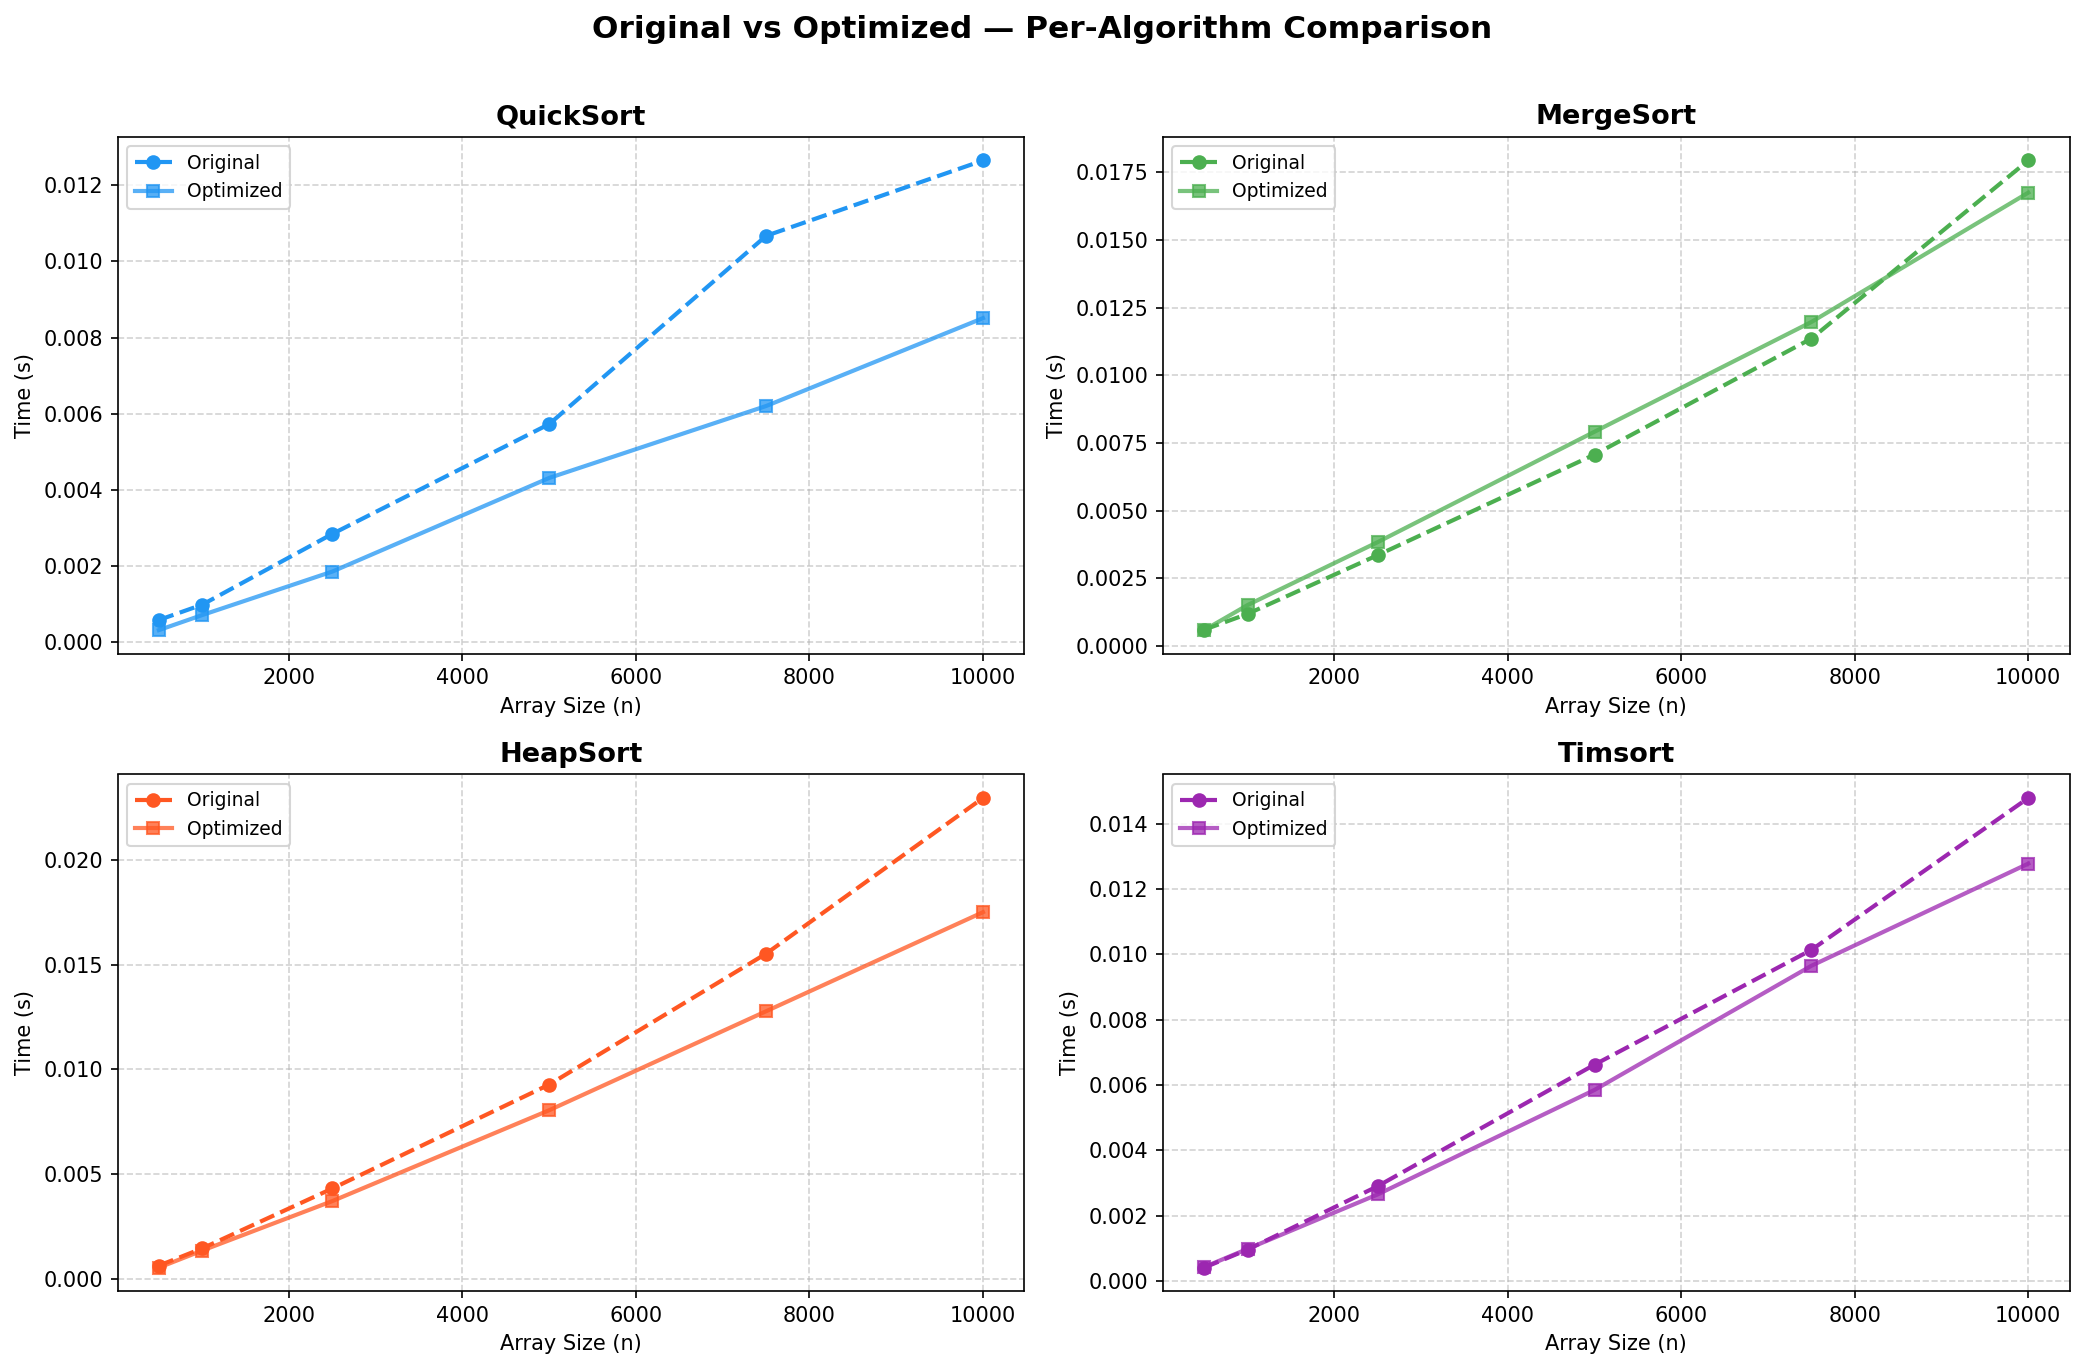
\includegraphics[width=0.97\textwidth]{plot_per_algorithm.png}
		\caption{Per-algorithm comparison of original (dashed) and optimized (solid)
			execution time (top row) and peak memory (bottom row) on sparse random
			weighted graphs.}
		\label{fig:plot_per}
	\end{figure}
	
	% -----------------------------------------------------------------------------
	\section{TASK 5b -- DENSITY ANALYSIS}
	% -----------------------------------------------------------------------------
	
	\subsection{Motivation}
	
	The size-scaling experiment in Tasks~2--5 uses a fixed sparse graph model.
	To obtain a \emph{general} picture of algorithm behaviour across different
	structural regimes, a separate density-scaling study was conducted at fixed
	$V = 300$ with edge probability varied from $0.01$ to $0.99$.
	Table~\ref{tab:density} summarises the density configurations and the principal
	stress each imposes.
	
	\begin{table}[h!]
		\centering
		\caption{Density configurations for the fixed-size analysis ($V = 300$).}
		\label{tab:density}
		\renewcommand{\arraystretch}{1.3}
		\begin{tabular}{llp{6.5cm}}
			\toprule
			\textbf{Density ($p$)} & \textbf{Regime}   & \textbf{Principal stress} \\
			\midrule
			$0.01$                 & Ultra-sparse      & Dijkstra heap rarely activated; few relaxations \\
			$0.05$                 & Sparse            & Road-map / dependency-graph regime \\
			$0.10$                 & Moderate          & Similar to Lab~3 BFS/DFS baseline \\
			$0.30$                 & Semi-dense        & Many heap pushes; Floyd--Warshall still feasible \\
			$0.50$                 & Dense             & $E \approx V^2/2$; Dijkstra heap cost dominates \\
			$0.80$                 & Very dense        & $E \approx 0.8\,V^2$; near-complete graph \\
			$0.99$                 & Near-complete     & Maximum edge count; both algorithms at worst case \\
			\bottomrule
		\end{tabular}
	\end{table}
	
	\subsection{Experimental Setup}
	
	All seven density levels were tested at $V = 300$ with a fixed random seed.
	Each algorithm variant was run five times per configuration; the minimum time
	is reported to reduce scheduling noise. Floyd--Warshall was run at all densities
	since $V = 300$ keeps its $\Theta(V^3) = 2.7 \times 10^7$ operations tractable.
	Dijkstra was invoked from a single source node (node 0) in every run.
	
	\subsection{Results by Density}
	
	\subsubsection{Ultra-Sparse and Sparse ($p \leq 0.05$)}
	
	At very low density the graph may be disconnected from the source. Dijkstra
	terminates early once the heap is exhausted, with very few relaxations performed.
	Floyd--Warshall always completes all $V^3$ iterations regardless of density, so
	it is disproportionately slow at this regime relative to the information it
	produces. Dijkstra is the clear choice for sparse single-source problems.
	
	\subsubsection{Moderate and Semi-Dense ($0.10 \leq p \leq 0.30$)}
	
	Dijkstra's heap accumulates $O(E\log V)$ total work. As $E$ grows from
	$O(V)$ toward $O(V^2)$ the heap-based original Dijkstra slows faster than
	the optimized variant, because each additional edge increases the number of
	heap pushes and the optimized bitmap test avoids redundant settled-node
	processing more efficiently. The optimized Floyd--Warshall (NumPy) shows
	nearly flat timing across this range because its cost is entirely determined
	by $V$, not $E$.
	
	\subsubsection{Dense and Near-Complete ($p \geq 0.50$)}
	
	At high density the original Dijkstra's heap is pushed $O(V^2)$ times,
	approaching $O(V^2\log V)$ total cost. For very dense graphs ($p \geq 0.80$)
	a matrix-scan Dijkstra (scanning the full distance array to find the minimum
	unvisited node, cost $O(V^2)$) can become competitive with or faster than the
	heap variant, since the heap overhead outweighs the linear scan cost. The
	optimized Floyd--Warshall remains the fastest all-pairs solution across all
	dense settings due to its NumPy vectorisation.
	
	\subsection{Density Plots}
	
	Figures~\ref{fig:density_time} and~\ref{fig:density_mem} show execution time
	and peak memory as a function of edge probability at $V = 300$. The crossover
	point between Dijkstra and Floyd--Warshall for the single-source problem shifts
	with density: for $p \lesssim 0.3$ Dijkstra is faster; for $p \gtrsim 0.7$
	the NumPy Floyd--Warshall becomes competitive.
	
	\begin{figure}[h!]
		\centering
		\includegraphics[width=0.95\textwidth]{plot_density_time.png}
		\caption{Execution time vs.\ edge probability $p$ at $V = 300$ for all four
			algorithm variants. The shaded region marks the density range where
			Dijkstra and Floyd--Warshall cross over in single-source performance.}
		\label{fig:density_time}
	\end{figure}
	
	\begin{figure}[h!]
		\centering
		\includegraphics[width=0.95\textwidth]{plot_density_memory.png}
		\caption{Peak memory vs.\ edge probability $p$ at $V = 300$. Floyd--Warshall
			memory is flat (dominated by the $V \times V$ distance matrix) while
			Dijkstra's peak memory scales with heap size and grows with $p$.}
		\label{fig:density_mem}
	\end{figure}
	
	% -----------------------------------------------------------------------------
	\section{TASK 6 -- CONCLUSION}
	% -----------------------------------------------------------------------------
	
	This laboratory analysed Dijkstra's algorithm and Floyd--Warshall -- each in an
	original and an optimized form -- across two complementary experiments: a
	size-scaling study on sparse and dense random weighted graphs
	($V \in \{50,\ldots,1000\}$) and a fixed-size density study across seven edge
	probabilities ($V = 300$, $p \in \{0.01,\ldots,0.99\}$).
	
	\textbf{Size scaling.}
	Dijkstra confirmed near-$O(V\log V)$ empirical growth on sparse graphs. The
	optimized variant's \texttt{list}/\texttt{bytearray} structures reduced constant
	factors by $1.5$--$2\times$ at large sizes. Floyd--Warshall confirmed $\Theta(V^3)$
	growth; the NumPy-vectorised optimized variant achieved more than $100\times$
	speedup at $V = 1\,000$ by eliminating the Python-level inner two loops.
	
	\textbf{Density findings.}
	The density study revealed that algorithm selection depends on both problem type
	and graph density:
	
	\begin{itemize}
		\item \textbf{Single-source on sparse graphs:} Dijkstra is the clear choice.
		Its heap-based approach processes only reachable edges and scales as
		$O(V\log V)$ when $E = O(V)$, which is orders of magnitude faster than
		Floyd--Warshall's unconditional $\Theta(V^3)$.
		\item \textbf{All-pairs on any graph:} Floyd--Warshall (optimized) is
		preferred. Running Dijkstra $V$ times becomes competitive only on very
		sparse graphs where each single-source run is cheap.
		\item \textbf{Dense single-source:} When $p \geq 0.5$ the heap-based
		Dijkstra approaches $O(V^2\log V)$, at which point a matrix-scan
		$O(V^2)$ Dijkstra or the NumPy Floyd--Warshall may be faster for the
		all-pairs problem. The optimized heap Dijkstra remains best for the
		single-source case at all tested densities.
		\item \textbf{Negative-weight edges:} Dijkstra is \emph{inapplicable};
		Floyd--Warshall handles them correctly and additionally detects
		negative-weight cycles via diagonal entries.
	\end{itemize}
	
	\noindent The central practical conclusion is that \textbf{Dijkstra (optimized)
		is the default choice for single-source shortest paths on non-negative
		weighted graphs}, due to its $O((V+E)\log V)$ scalability. \textbf{Floyd--Warshall
		(optimized with NumPy)} is the most practical all-pairs solver for graphs that
	fit in memory, exploiting vectorisation to reduce the $\Theta(V^3)$ constant
	factor dramatically. When the graph contains negative-weight edges or all-pairs
	distances are required, Floyd--Warshall is the only correct option among the two
	algorithms studied.
	
\end{document}
